% !TeX root = main.tex
\graphicspath{{figures/}}
\lecture{3}{Wed 08 Oct 2025 11:00}{Generalised Wavefunctions}

Recap: For a sine wave, the wavefunction is:
\[
    y(x,t) = A \cos(kx - \omega t)
\]
Where k is the wave number, $k = \frac{2 \pi}{\lambda}$ and omega is $\frac{2 \pi}{T} = 2 \pi f$

\section*{More Wavefunctions}
What is the general form of a triangular shaped wave? What about a square stepped wave?
TODO: Diagram

We know that each particle (i.e. along a string) copies the motion of its immediate left-hand neighbour (for a particle moving in the positive x), with a time delay proportional to their distance. Every wave is describable $y(x,t)$ wave function, and every mechanical wave relies on a medium (i.e. a piece of string or water, concrete etc) to travel.

Ideally, we want to be able to find a general form of a wave function.

In a single fixed instant of time, the moving wave pulse is stationary, so purely a function of $y = f(x)$. We want a wave function where we can input any value of $t$, so we need a moving frame of reference. We define this frame of reference as $O'$ (for the origin) and $x', y'$ axes. This frame of reference moves with the wave pulse and at the same speed, therefore y' is a function of x' only, independant of speed.

\subsection*{New System}
$x$ is the distance from the origin $O$ to the relevant point, while $x'$ is the distance from $O'$.

\[
    x = x' + vt
\]

\[
    x' = x - vt
\]

\[
    y' = f(x') = f(x-vt)
\]

However, as the wave is moving purely in one direction (along x), $y = y'$, so:
\[
    y = f(x - vt)
\]


\subsection*{Back to Basics}
Going back to:
\[
    y(x,t) = A \cos(kx - \omega t)
\]
\[
    = A \cos\left[k\left(x - \frac{\omega}{k}t\right)\right]
\]
\[
    = A \cos\left[k\left(x - vt\right)\right]
\]
(Note, this is true for a wave in the positive x, for a wave moving in the negative x this would be x + vt)


\subsection*{Equivalent Rrepresentations}
There are some equivalent representations for a sine wave:
\[
    y(x,t) = A \cos \left(2 \pi f \frac{x}{v} - \omega t\right) = A \cos\left(2 \pi \left[\frac{x}{\lambda} - \frac{t}{T}\right]\right) = TODO
\]

\section*{More Differentiation}
We've already looked at differentiating with respect to t, but what about x? This would give us the slope of the string at that point:

\[
    \frac{\partial y(x, t)}{\partial x}
\]

And the curvature of the string:
\[
    \frac{\partial^2 y(x, t)}{\partial x^2} = -k^2 A \cos(kx - \omega t) = -k^2 y(x, t)
\]
Note the similarities here with the equation for transverse acceleration:


\begin{equation*}
    (1) \frac{\partial^2y(x, t)}{\partial t^2} = -\omega^2 y(x, t)
\end{equation*}

\begin{equation*}
    (2) \frac{\partial^2 y(x, t)}{\partial x^2} = -k^2 y(x, t)    
\end{equation*}

Dividing (1) by (2):

\[
    \frac{\partial^2y(x, t) / \partial t^2}{\partial^2 y(x, t)/\partial x^2} = \frac{\omega^2}{k^2} = v^2
\]

Therefore:
\[
    \frac{\partial^2 y(x, t)}{\partial x^2} = \frac{1}{v^2} \frac{\partial^2 y(x, t)}{\partial t^2}
\]
We call this the `wave equation' as every wave function y(x, t) must satisfy it, regardless of whether or not it is periodic or its direction of travel. If y(x, t) does not satisfy this, it is not a wave function.


\subsection*{An Example}
\[
    y(x, t) = \frac{x^3 - vt^2}{e^t}
\]
TODO, the example in our own time

\section*{Wave Equation for a String}

\begin{figure}[H]
    \centering
    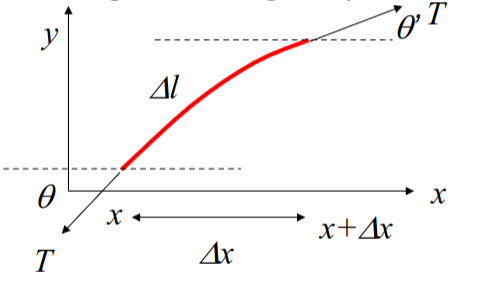
\includegraphics{figures/lec03-02.png}
     \caption{A snapshot of the wave.}
\end{figure}


Lets say we have some string, suspended horizontally under tension. We generate a single wave pulse and allow it to propogate down the string.

We assume the string is 1D, under tension $T$ (constant throughout) and has mass per unit length $\mu$.

Consider a small segment of string of length $\Delta L$ from $x$ to $x + \Delta x$. This string makes angle $\theta$ with the horizontal at the bottom of the string, and angle $\theta'$ with the horizontal at the top of the string.

Net force is:
\[
    F_y = T \sin \theta' - T \sin \theta
\]

And using the small angle approx $\sin \theta \approx \tan \theta = \frac{dy}{dx}$:

\[
    F_y = T\left(\frac{dy}{dx} \Bigr\rvert_{x + \Delta x} - \frac{dy}{dx} \Bigr\rvert_{x}\right)
\]

Using differentiation by first principles:
\[
    \frac{dy}{dx} = \lim_{\Delta x \to 0} \frac{f(x + \Delta x) - f(x)}{\Delta x}
\]


We can say:
\[
    \frac{d^2y}{dx^2} = \frac{d}{dx}\left(\frac{dy}{dx}\right) = \lim_{\Delta x \to 0} \frac{\frac{dy}{dx} \Bigr\rvert_{x + \Delta x} - \frac{dy}{dx} \Bigr\rvert_{x}}{\Delta x}
\]

Therefore:
\[
    F_y = T \frac{d^2y}{dx} \Delta x
\]



